% Chapter Template

\chapter{ Study of the internal structure of a previously trained Recurrent Neural Network} % Main chapter title

\label{Chapter 3} % Change X to a consecutive number; for referencing this chapter elsewhere, use \ref{ChapterX}

\lhead{Chapter 3. \emph{Study of the internal structure of a previously trained Recurrent Neural Network}} % Change X to a consecutive number; this is for the header on each page - perhaps a shortened title

%----------------------------------------------------------------------------------------
%	SECTION 1
%----------------------------------------------------------------------------------------

%\section{State of the Art}

\section{Motivation}

In this chapter we study the internal structure of an example of previously trained recurrent neural networks in order to propose a practical improvement of the architecture for a given problem. The lack of understanding of the dynamics within a neural network and the progress of computation performance and implementation of Neural Netowrks led to accepting that the larger the network is, the better it is suited to obtain a better solution. Many techniques have been implemented in order to reduce the overfitting of these models that contains a large number of parameters such as Georges Hinton's dropouts for training Deep Feed-Forward Neural Networks. However, it seems rather unnatural to ommit the study of the internal structure of a network in the field of Deep Learning and especially for Recurrent Neural Network, where complex dynamics of the states can be observered. For example, in the classical model of a Recurrent Neural Network, the weight matrix is dense but if we observe the human brain, it is estimated that the number of neurons is approximatively $10^{11}$ and the number of synapses between $10^{14}$ and $10^{15}$, which means that the mean number of connections from a neuron to another is between $10^3$ and $10^4$ and therefore that the weight matrix is extreamly sparse. In this chapter we use graph theory techniques to perform an empirical study of a neural networks that has been previously trained with a memory problem. 

\section{Experiments}

\subsection{Problem}

The neural network is trained on a 100 timestep sequence of random binary numbers, where the goal is to memorize the first input given to the network. It contains 100 neurons and it is trained using the Hessian Free Optimization method (HFO). This example use the Theano implementation of the HFO of Boulanger-Lewandowski \cite{boulanger2012modeling}. The network was trained for approximatly 8 hours on a 4 cores computer which gave a 0 error on the validation set as described on the Github repository of Boulanger-Lewandowski. In the end of the training we obtain the (100, 100) hidden-to-hidden weight matrix and perform the graph analysis on this matrix. This kind of memorization problem is typically hard for a recurrent neural network to learn, when its trained using stochastic gradient descent because it emphasizes the vanishing gradient problem. The relevant input is 100-timestep old, and therefore the weight matrix is multiplied a 100 times, before reading the output which will be small as a composant of the gradient. Therfore this problem demonstrates the importance of a 2-order optimization method for RNNs. 

\subsection{Plot of the RNN}

In order to display the RNN, we use two differents layouts, the nodes are represented with red dots, the connection are in blue when $w_{ij}  > t $ where t is a threshold ($ t=0.15$ for the following figures) and in black when $w_{ij} < - t$  :

\begin{itemize}
    \item The spring layout, where the positions of the nodes is calculated as if each connection was a spring which rigidity constrain is the weight of the connection ( or 2 particles with opposite charge for a negative weight. ) (ie minimizing the energy $$ E(x, y) = \sum_{i,j} w_{ij}(\sqrt{(x_i - x_j)^2 + (y_i - y_j)^2} - l)^2 $$ where $l$ is the default length of a connection. 
    \item The spectral layout \cite{koren2003spectral} that performs eigenanalyses of the Laplacian Matrix ($L$) of the Graph and uses the eigenvectors of L to display the nodes on the 2D plane. L is defined as $$ L = D - A $$ where A is the symmetrical Matrix $$ A = 0.5(W + W^\top) $$ (because the RNN is a directed Graph.) and D is the diagonal matrix such that :  $$ D_{ii} = \sum_j A_{ij} $$ 
        $L$ is a semi-definite symmetrical Matrix with zero row sums. Therefore there is a spectral decomposition of this Matrix with positive eigenvalues and its eigenvectors are orthogonal. The two (or more for a n-dim layout) eigenvectors corresponding to the smallest non-zero eigenvalues are kept and use as the x and y coordinates.  

        The Laplacian matrix has the following property : $$x^\top  L x = \sum_{i < j} A_{ij}(x_i - x_j)^2 $$
        Displaying the graph as follow is the solution of a minimization problem ie : For a 1-D layout minimizing the energy $E$ defined as follow : 
        $$ E(x) = \sum_{i,j} A_{ij} (x_i - x_j)^2 $$ where $x \in \mathbb{R} $ with a constrain on the variance of $x$ : $Var(x) = 1 $. 
        Minimizing this energy with a fixed variance will tend to make the edges as small as possible (with respect of the weights) and prevent all nodes to be on the same position. 
    This problem is equivalent to the following (when placing the mean of x to be null) : 
    $$ min_x x^\top L x $$
    given $ x^\top x = 1 $
    on the hyperplane $x^\top \dot 1_n = 0 $

    which corresponds to setting x to be the smallest normalized eigenvectors ($v_1$) (ie corresponding to the smallest non-zero eigenvalue) of L.
    The same reasonning can be applied to obtaining a k-dim layout, as the eigenvectors are orthogonals, we can resolve the same minimisation problem on the the subspace orthogonal to $v1$ for the second dimension ( which will be taking $y = v_2$) and so on. 
\end{itemize}


\begin{figure}[htbp]
    \centering
    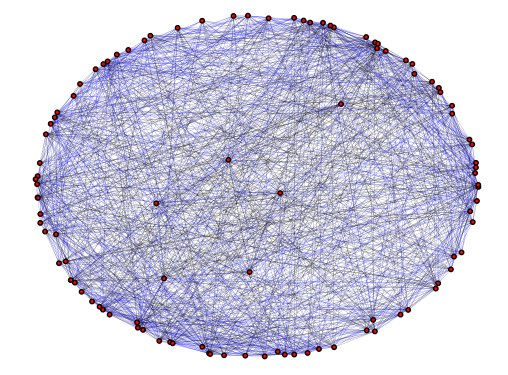
\includegraphics[scale=0.8]{Figures/weighted_graph_spring.png}
    \rule{35em}{0.5pt}
    \caption[Plot of the RNN using weights as springs]{Plot of the RNN using weights as spring}
    \label{fig:ring_lattice}
\end{figure}


\begin{figure}[htbp]
    \centering
    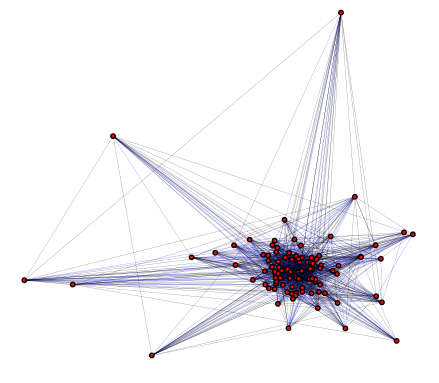
\includegraphics[scale=0.8]{Figures/weighted_graph_spectral.png}
    \rule{35em}{0.5pt}
    \caption[Plot of the RNN with spectral analyses of the Laplacian Matrix ]{Plot of the RNN with spectral analyses of the Laplacian Matrix}
    \label{fig:ring_lattice}
\end{figure}

We can observe that 5 nodes are on the periphery of the spectral graph, which means that they have small connections to the rest of the nodes (ie no strong connection to a cluster), whereas the other nodes have neighbors "strongly" attached to them. 

\subsection{Weight distribution}
It is also interesting to display the weight distribution : 

\begin{figure}[htbp]
    \centering
    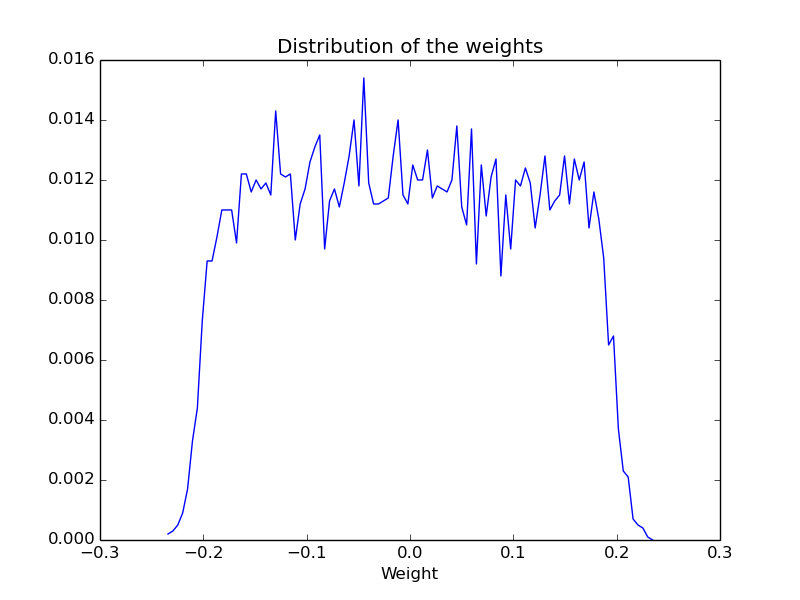
\includegraphics[scale=0.4]{Figures/weight_distribution.png}
    \rule{35em}{0.5pt}
    \caption[Weight distribution ]{Weight distribution}
    \label{fig:weight_dist}
\end{figure}

\begin{figure}[htbp]
    \centering
    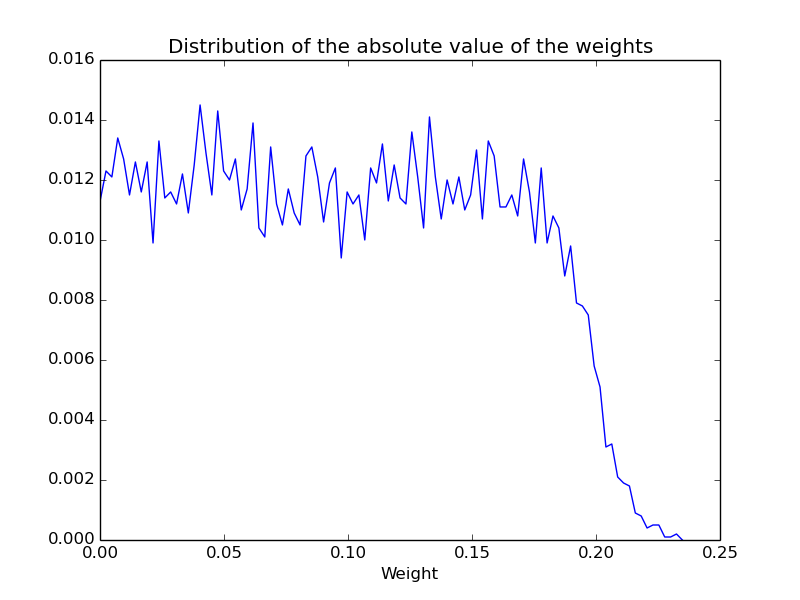
\includegraphics[scale=0.4]{Figures/abs_weight_distribution.png}
    \rule{35em}{0.5pt}
    \caption[Distribution of the absolute value of the weights]{Distribution of the absolute value of the weights}
    \label{fig:abs_weight_dist}
\end{figure}

We can observe a that the distribution is relativly symmetric and that most weights are within the interval $[-0.2;02] $

\subsection{Sums of weights}

It is also interesting to compute the sum of the absolute value of the weights of the input connections in the hidden matrix ( ie : the rows of $W_{hh}$) ($\sum_{in,}(Whh)$) and also the output connection ($\sum_{out,}(Whh)$) (ie the columns of t $W_{hh} $). A neuron without any influence on the network has ($\sum_{out,}(Whh) = 0$) and a neuron which state is constant has the $\sum_{in,}(Whh) = 0$. Therefore by studying this 2 sums, we can hope to determine if some neurons are useless, or in the opposite if one neuron should be cloned.
The following figures are the plot of these sums on the network. 

\begin{figure}[htbp]
    \centering
    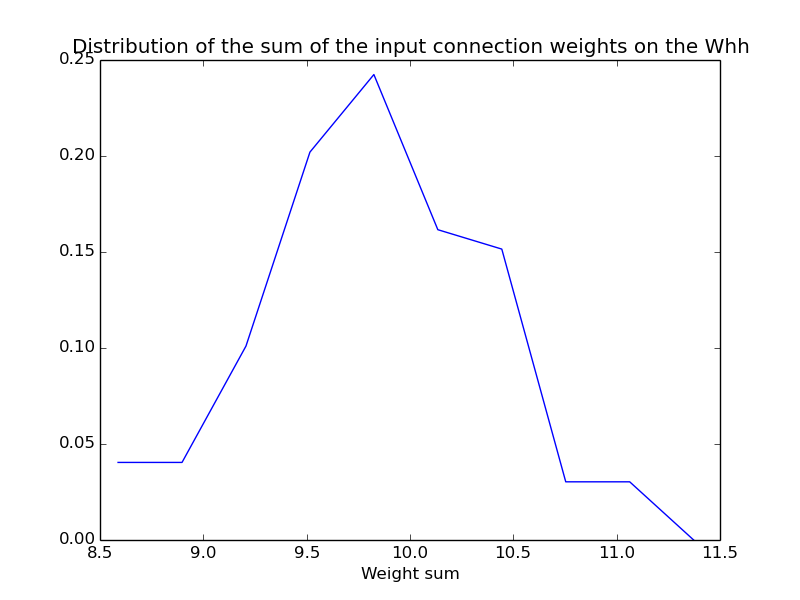
\includegraphics[scale=0.4]{Figures/input_sum_weight_distribution.png}
    \rule{35em}{0.5pt}
    \caption[Distribution of the sum of the input connection weights on Whh]{Distribution of the sum of the input connection weights on Whh}
    \label{fig:input_sum}
\end{figure}


\begin{figure}[htbp]
    \centering
    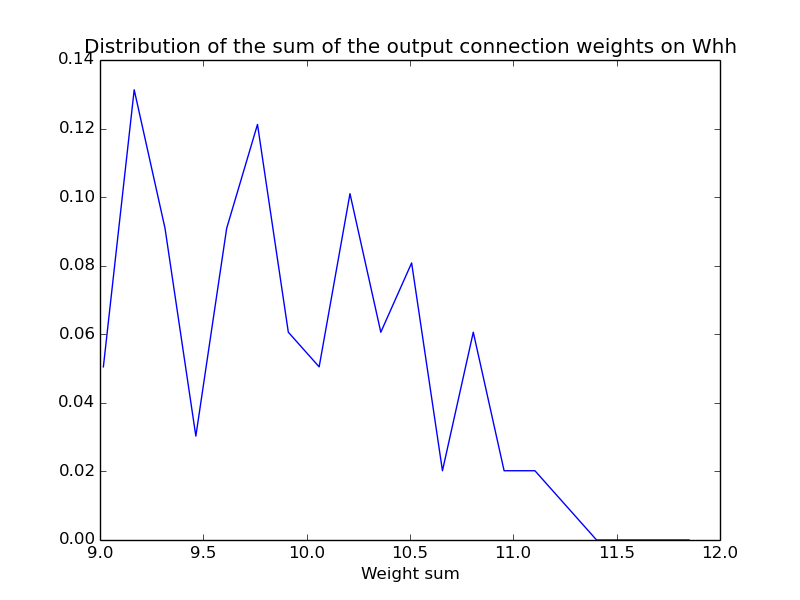
\includegraphics[scale=0.4]{Figures/output_sum_weight_distribution.png}
    \rule{35em}{0.5pt}
    \caption[Distribution of the sum of the output connection weights on Whh]{Distribution of the sum of the output connection weights on Whh}
    \label{fig:output_sum}
\end{figure}

A surprising result is that these two sums do not change as much as expected over the set of neurons : for all the neurons these two sums are within $[8.0; 12.0]$, it is therefore difficult two establish which neuron to remove based on this measure.

\newpage

\section{Results : comparing neurons of the network.}

We can also directly measure the impact of a neuron on the network. By replacing all the input and output weights of the neuron with zeros, we destroy its impact on the RNN. It is then possible to test the network on a validation set of sequence. We then display the results, that represent the percentage of errors on the validation set. 

\begin{figure}[htbp]
    \centering
    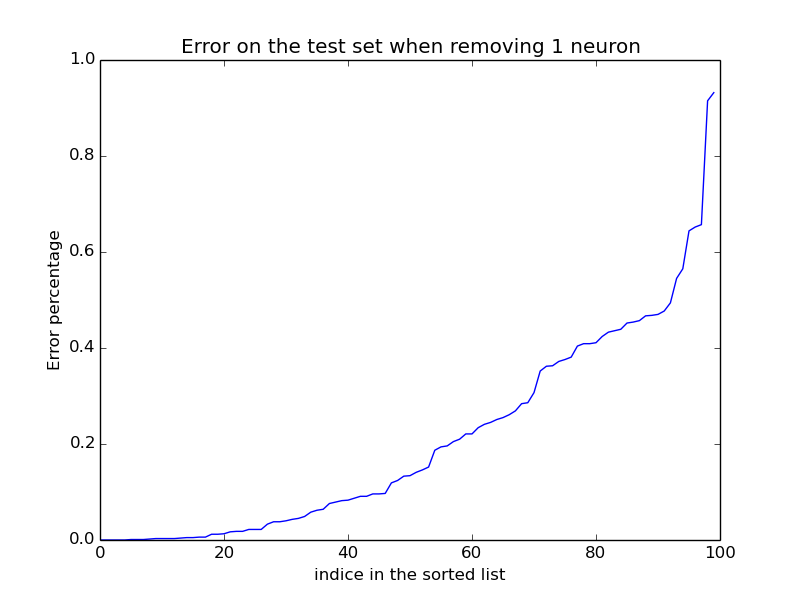
\includegraphics[scale=0.8]{Figures/error_test_set_remove_neuron.png}
    \rule{35em}{0.5pt}
    \caption[Error on the test set when removing 1 neuron]{Error on the test set when removing 1 neuron}
    \label{fig:error_one_neuron}
\end{figure}

In the figure \ref{fig:error_one_neuron} we display the sorted list of percentage error on the test set when removing 1 different neurons at each time. This figure demonstrate that the importance of the neurons in the network is very unequal. For $20$ neurons out of $100$, the network without this neuron the error rate will not exceed $3\%$ whereas if we remove only $1$ "important" neuron in the top $20$ , the network will have lesser performance than random guess ! This shows that the dynamics within a network can be perturbed easily only with a small modification of the architecture if this modification affects the wrong neurons. Another really interesting results that this graph shows is that the sum of the weights does not give a good approximation of the importance of a neuron's worth.

Using this measure, we can introduce an order relation $O$in the set of neuron : 

$$ N_i <= N_k \Leftrightarrow m(N_i) <= m(N_j) $$ where $m$ is a function that return the error percentage on the test set when removing a the neuron of the network.

In the following we compare this order relation with the ones obtained using other intrinsic metrics of the network. The goal is to find a way of knowing which neurons to remove in the network without "breaking" the dynamics involved so that the network is more efficient. In order to compare a metric with $m$ we sort the set of neurons and compare the list of indices. 

$$ d(s , s') =  \sum_{i \in \mathbb{N}} {| s_i - s'_i|} $$

A low value of $d$ means that 2 metrics order the neurons similarly. Using $d$ with the previously defined order relation provides a benchmark for finding an approximation of the worth of a neuron in the network. In the following we present the results of different metrics on this benchmark.

The metrics that were tested on the network are : 
\begin{itemize}
    \item M1 : The sum of the absolute value of the in an out weights on the hidden-to-hidden connection
    \item M2 : The sum of the in an out weights on the hidden-to-hidden connection
    \item M3 : The absolute value of the sum of the in an out weights on the hidden-to-hidden connection
    \item M4 : The clustering index
    \item M5 : The absolute value of the ouput weights ( of the hidden to output matrix) 
    \item M6 : The absolute value of the input weights ( of the hidden to output matrix) 
    \item M7 : The sum of the two previous metrics.
\end{itemize}
\newpage

All the metrics were normalized to be able to plot them with $m$.
In the following graphs we ploted the metrics for the sorted list of neurons with $O$, as well as the value of $m$. 


\begin{figure}[!htb]
    \centering
    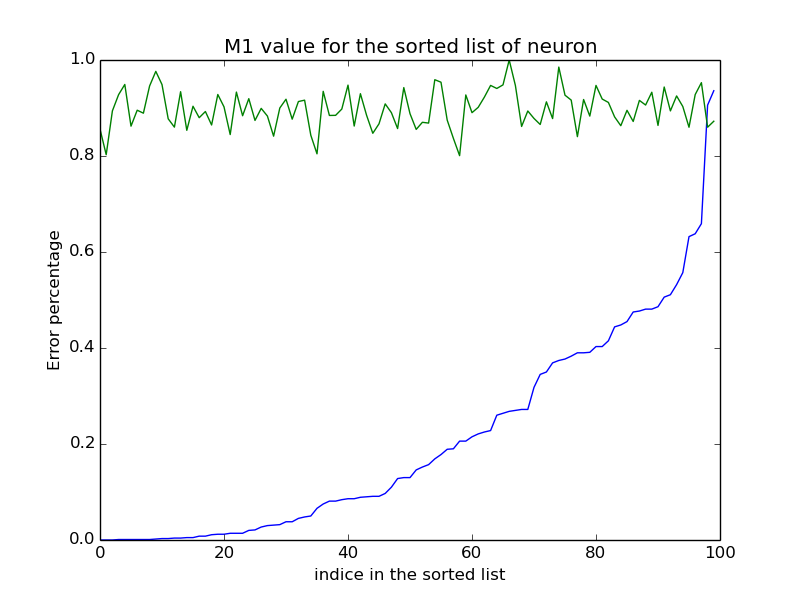
\includegraphics[scale=0.5]{Figures/m1.png}
    \rule{35em}{0.5pt}
    \caption[M1]{M1}
    \label{fig:m1}
\end{figure}


\begin{figure}[!htb]
    \centering
    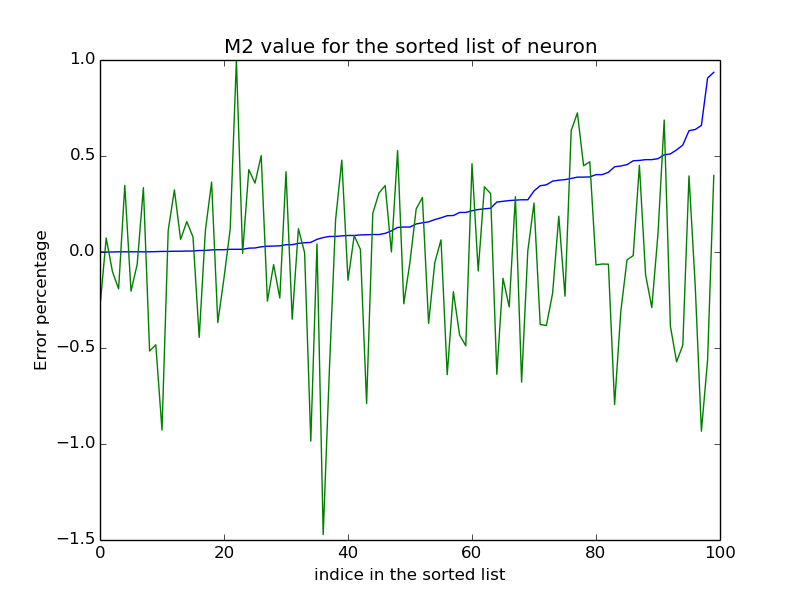
\includegraphics[scale=0.5]{Figures/m2.png}
    \rule{35em}{0.5pt}
    \caption[M2]{M2}
\label{fig:m2}
\end{figure}


\begin{figure}[!htb]
    \centering
    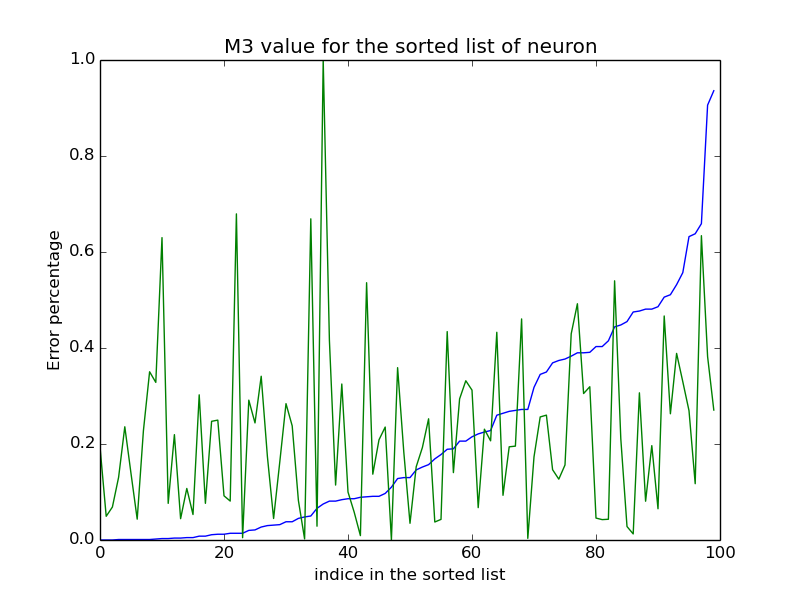
\includegraphics[scale=0.5]{Figures/m3.png}
    \rule{35em}{0.5pt}
    \caption[M3]{M3}
    \label{fig:m3}
\end{figure}


\begin{figure}[!htb]
    \centering
    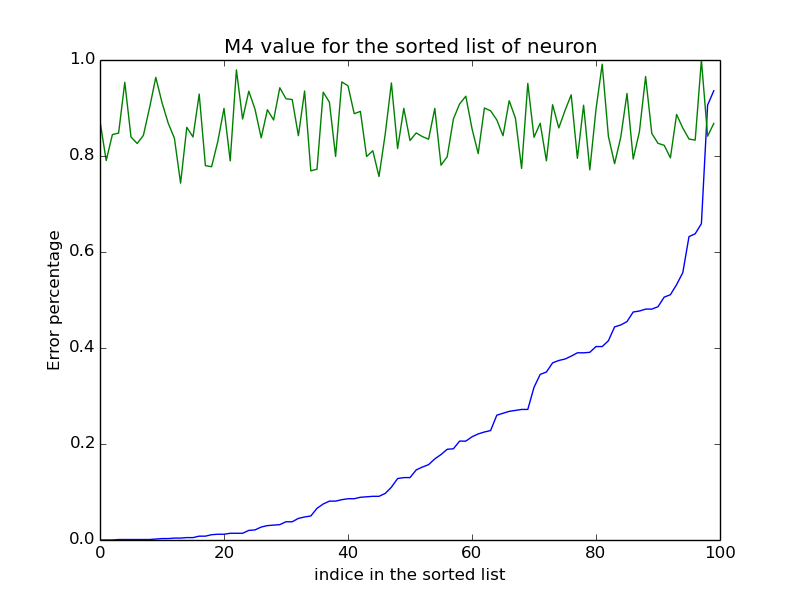
\includegraphics[scale=0.5]{Figures/m4.png}
    \rule{35em}{0.5pt}
    \caption[M4]{M4}
    \label{fig:m4}
\end{figure}


\begin{figure}[!htb]
    \centering
    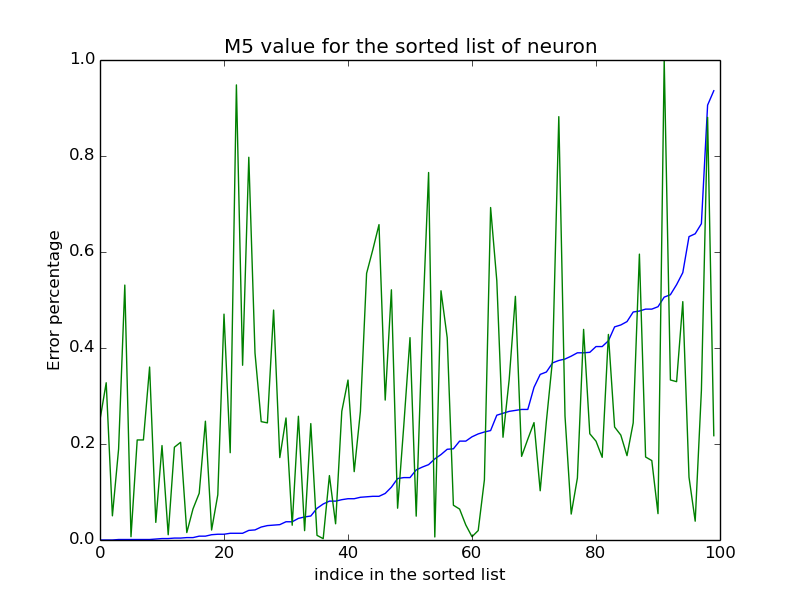
\includegraphics[scale=0.5]{Figures/m5.png}
    \rule{35em}{0.5pt}
    \caption[M5]{M5}
    \label{fig:m5}
\end{figure}


\begin{figure}[!htb]
    \centering
    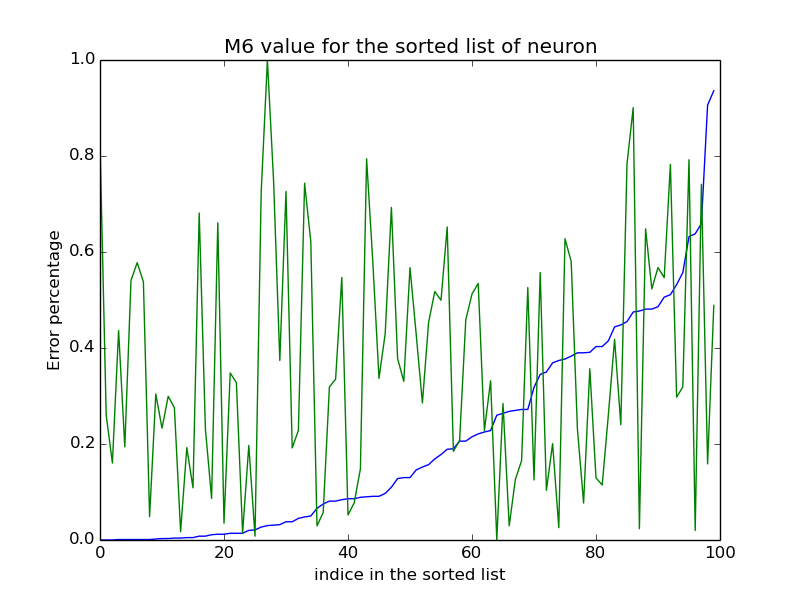
\includegraphics[scale=0.5]{Figures/m6.png}
    \rule{35em}{0.5pt}
    \caption[M6]{M6}
    \label{fig:m6}
\end{figure}


\begin{figure}[!htb]
    \centering
    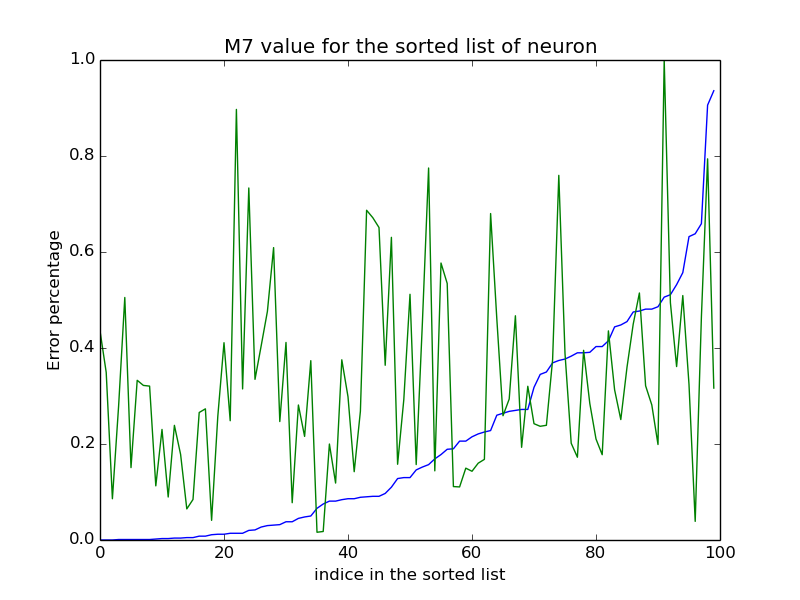
\includegraphics[scale=0.5]{Figures/m7.png}
    \rule{35em}{0.5pt}
    \caption[M7]{M7}
    \label{fig:m7}
\end{figure}

\newpage

In order to make the figure \ref{fig:m4} we use the local clustering coefficient. This coefficient describe how close the neighbors of a neuron are to forming a complete graph. In this case, as the graph is using weighted connection, it represents how tied together are its neighbors. 

\newpage

\begin{figure}[!htb]
    \centering
    \begin{tabular}{|l|l|}
        \hline
        M1 & 3118 \\ \hline
        M2 & 3294 \\ \hline
        M3 & 3512 \\ \hline
        M4 & 3388 \\ \hline
        M5 & 3244 \\ \hline
        M6 & \textbf{2944} \\ \hline
        M7 & 3402 \\
        \hline
    \end{tabular}
    \label{fig:metrics}
    \rule{35em}{0.5pt}
    \caption[Table presenting the value of d for the different metrics ]{Table presenting the value of d for the different metrics}
\end{figure}

From these results we can conclude that though these indicators seem "natural" to provide a good estimation of which neuron is important within the network, it is not the case. Therfore, for the follwing work, we use a validation dataset to obtain the "worth" of a neuron. However, It would be interesting to construct such an indicator that could perform this task without testing the network on data, but directly from the structure of the network (see Conclusion and Future Work).




\section{Results: Comparing connections in the network.}

In this section we perform the same analyse on weighted connections. By removing the connections one by one, and testing the network on a validation dataset, we obtain a score for each connection. This calculation is in complexity comparable to the number of connexions, which is $n ^2$ for a classical dense RNN. For this experiment we reduce the validation set size because of the complexity to a $1000$ sequences.


\begin{figure}[htbp]
    \centering
    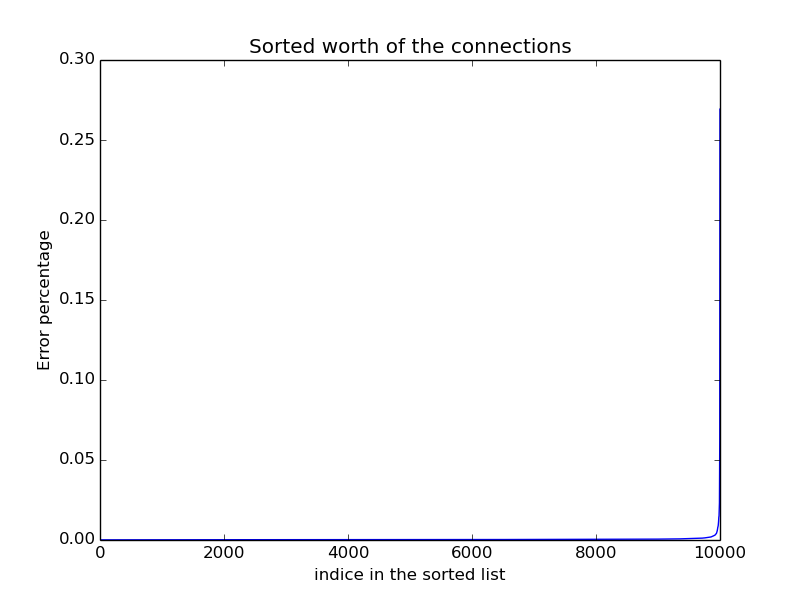
\includegraphics[scale=0.5]{Figures/score_worth_connection.png}
    \rule{35em}{0.5pt}
    \caption[Sorted Worth of the Connection]{ Sorted Worth of the connection}
    \label{fig:score_worth_connection}
\end{figure}

The first thing we can observe in figure \ref{fig:score_worth_connection} is that in a dense trained network, many connections don not harm the results of the network when we remove them. This confirm the intuition inspired from biology that was stated in the Introduction. A large subset of the weight connections have almost no influence on the results of the network. On this particular example, $9638$ connections out of $10000$ have less than $0.001$ change on the loss. 


\begin{figure}[htbp]
    \centering
    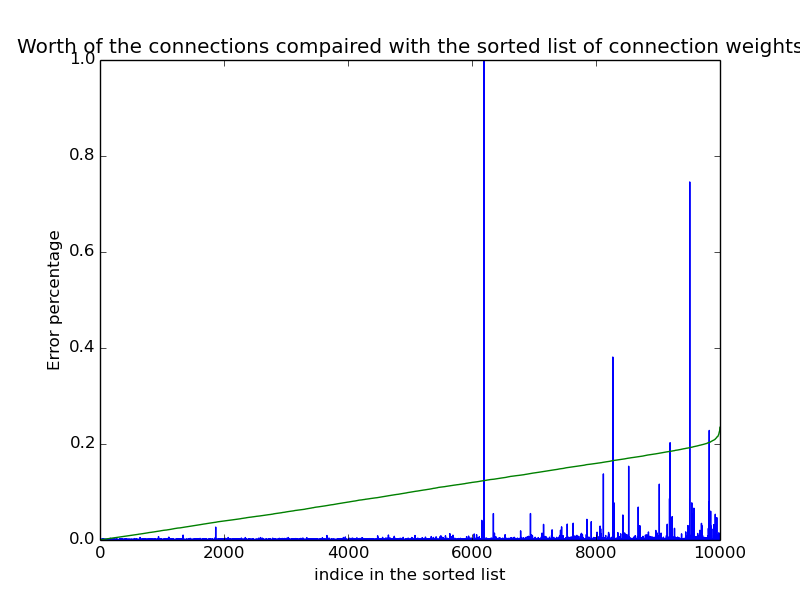
\includegraphics[scale=0.5]{Figures/score_vs_weight_connections.png}
    \rule{35em}{0.5pt}
    \caption[Score Vs Weigth of the connections]{Score vs Weight of the connections}
    \label{fig:score_vs_weight}
\end{figure}

On figure \ref{fig:score_vs_weight}, we ploted in blue the score and in green the absolute value of the weight of the sorted list of connections (sorted using the weights.). On this graph we can observe that having a small absolute value of weight makes the connection less important (There is less noise on the left part of the graph). However having a large weight, even if it is a necessary condition does not necessary mean that the connection is important. 

It would be an interesting result to compare the "important" neurons and the "important" connections, to see if it is possible to approximate the worth of connection using the weight and the worth of the neurons it connects (See Conclusion and Future Work) 
